

To study memory concurrency in commodity systems and begin building a runtime, we did experiments that approximate large irregular applications. The experiments consist of multiple threads each walking a number of separate linked lists. Each memory reference of a node is highly likely to result in an access to main memory, and we control the number of concurrent requests offered by a thread by varying the number of lists each thread walks. \todo{Brandon: somewhere we might explicitly say that this experiment involves no synchronization on list nodes, and relate to plan to build this as mentioned in the components of runtime section} Our experiments were run on a Xeon X5660, which uses the Nehalem microarchitecture, and has 2 sockets, 6 cores per socket, and 12GB of DRAM per socket. For the results listed, memory allocations were pinned to the DRAM of the first socket (``socket0"). Memory references from cores of socket1 must be satisfied by sending requests over the QPI link between the sockets. \todo{Brandon: is it important to mention that for isolation we use huge pages to reduce TLB misses?}
\subsection{Results}
 
\todo{might also include simple bar graph with max 1 socket, max 2 sockets, to membind=0}


\todo{choose best phrase to use for outstanding/concurrent miss/refs/reads and use consistently unless there is a place one makes most sense}
	 Figure~\ref{fig:listwalk-totalconc} shows the total number of outstanding misses the system can handle before performance plateaus. We found that for a single core, bandwidth plateaus once there are 10 concurrent misses; this is because the L1 cache line-buffer, which keeps track of outstanding misses of the core, is size 10. If concurrency is limited, there is less latency tolerance and performance is limited. 

	Running multiple cores, the system reaches a bandwidth plateau with fewer outstanding misses per core. In fact, the maximum number of total memory references in flight on a single socket is consistently 36. When using all six cores on the socket, bandwidth peaks at about 275Mref/s (see Figure~\ref{fig:listwalk-maxrates}). Since this is less than even a conservative bound on available pin bandwidth to DRAM, there is some bottleneck to performance in the memory system. A likely place is the global read-tracker queue containing references to the L3 cache; it has a capacity of 32 references, which concurs with the observed limit of 36 in-flight references. In addition, we performed measurements using performance counters, which consistently showed an average queue occupancy of 27, also close to the capacity 32.
 \todo{Brandon: it is great to identify why the bandwidth is limited, but in paper need to connect to why it is important. in general, we get an idea of what might need to be changed, especially as latency goes up and we need more concurrency}  \todo{cite ``multi-socket memory concurrency" to validate bandwidth numbers}
	Bandwidth of memory requests from cores on a single socket seems to peak at about 275Mreq/s; however adding requests to socket0's memory from socket1 cores increases the bandwidth to about 350Mreq/s, showing that there is additional room in the memory system that is simply reserved for remote requests.\todo{Currently a bit of a 
hanging statement, but it is intended to show more evidence of limit being queue.}

%\begin{figure*}
%	\begin{center}
%		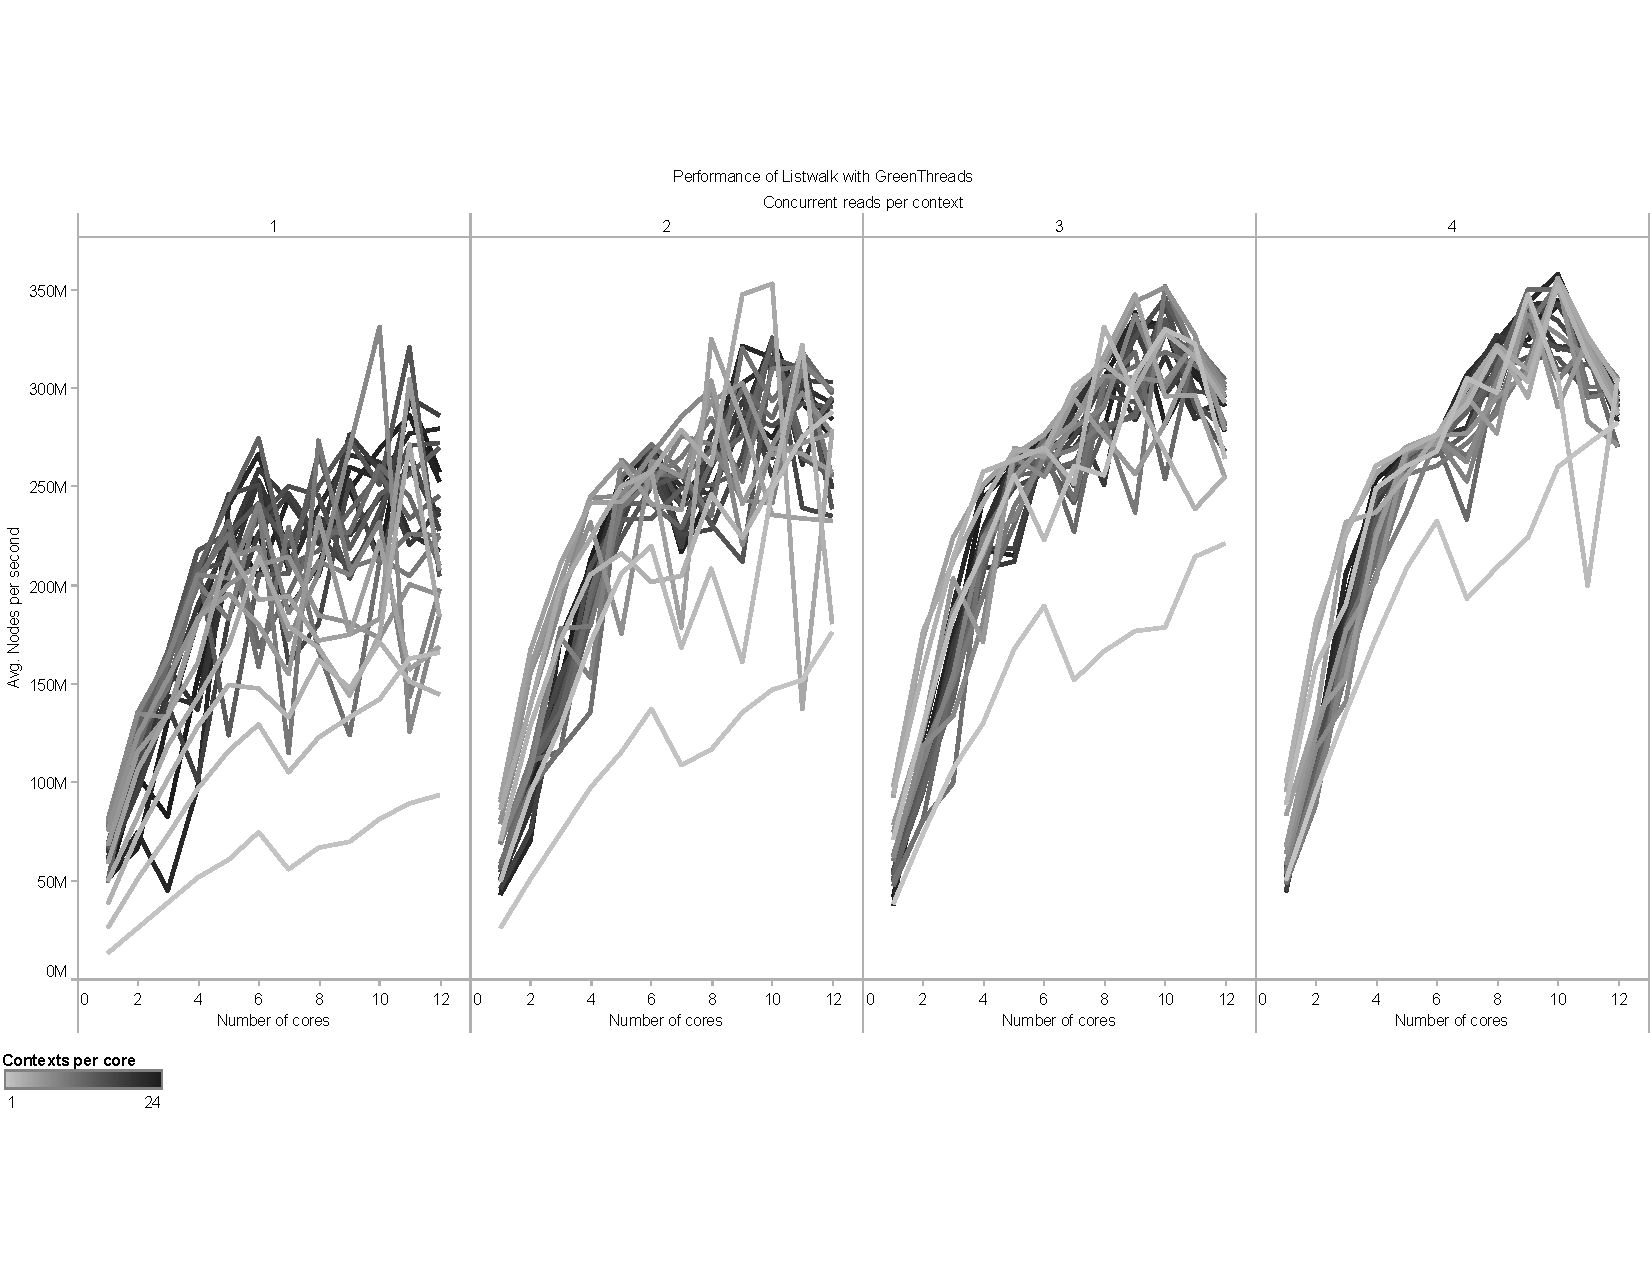
\includegraphics[width=0.5\textwidth]{figures/multi-core-green-thread-1gb.pdf}
%	\end{center}
%	\caption{}
%	\label{fig:listwalk-green-threads}
%\end{figure*}

\subsection{Using green threads}
	If a core is to have the number of concurrent memory requests required to tolerate latency and keep busy, it may need multiple contexts \todo{Brandon: this idea likely goes elsewhere in describing overall approach}.  We ran our experiments with varying numbers of green threads per core to use multiple contexts to achieve concurrency. Our results, displayed in Figure~\ref{fig:listwalk-green-threads} \todo{decide whether max/avg rate as well as how much info/whether to make consistent with the other plots format}, show that using green threads gives little to no overhead due to context switching. \todo{Brandon: somehow also tie in prefetch-and-switch; also might elaborate on the results and yield-only if space}


\subsection{Expanding to Multiple Compute Nodes}
	\todo{better title?}\\
	\todo{needs introduction, which will depend on what the system description section looks like}\\
	We use the single processor experiments to give insight into concurrency requirements in a multi-node system that uses a network with relatively long latency. 
	
	On the Nehalem, the QPI link to the network interface provides a bandwidth 12.8GB/s each way. This as much as 200Mref/s for 64-byte messages. For uniformly random distributed references across the entire shared memory space, we can expect half of this outgoing bandwidth will go towards satisfying remote requests, leaving half for making requests.  So, the cores can put out a bandwidth of 100Mref/s at full utilization of the link. Recent networks have suggested a max issue rate of 30M-90M messages per second is attainable \todo{cite mellanox press release and/or XT3/Eldorado} and this seems to be gradually increasing, so we use 100Mref/s as a good approximation to work with. Assuming a round-trip network latency of 1 to 2$\mu s$, then by Little's Law, the number of outstanding references is $(100Mref/s) * $(2 to 3 $\mu s$) = 200 to 300. This is the amount of memory concurrency that needs to exist for the latency of memory requests to be hidden when there is a rate of 100Mref/s.
We consider two issues: first, can we support 200-300 misses?, and second, can the caches support enough contexts? 
\todo{how many contexts required for that much memory concurrency.  Is it app dependent?} In order to keep the cores busy, there must be sufficient memory concurrency, and the number of contexts required to achieve this will vary. As there are more contexts in a core, there are more workings sets, including both data and coroutine stacks, that should fit in the cache to maintain performance.
	
	Can we support 200-300 misses? If the remote requests are reads that go to the global queue, then the number of outstanding references is limited to about 36. If the remote requests do not need to be stored in the global queue, then the line-fill buffers of the cores can support a total of $6 cores * 10 ref/core = 60 references$, still not quite enough. If, however, prefetches are messages--communicated with memory stores--requesting a piece of remote memory then many more outstanding references could be supported, either with a software data structure or a memory management device implemented in an FPGA.
	\begin{figure}[h]
	\begin{center}
 		\includegraphics[width=0.5\textwidth]{figures/multi-green-delay7800-edited.pdf}
	\end{center}
	\caption{}
	\label{fig:listwalk-green-delay}
\end{figure}
	We performed some experiments with green threads on listwalk, where we simulate the network latency by not allowing a coroutine to continue after it does a prefetch-and-switch until some specified amount of time has passed.  As seen in Figure \todo{ref delay plot} it is still possible to achieve the maximum throughput: it just requires more contexts to supply enough concurrent references, as expected. This simulation is of course limited both by the fact that prefetched data is actually sitting in cache longer than it should (increasing the effective working set size) and that the memory system still caps performance, but it is a useful validation of adding software contexts to achieve the level of concurrency that is necessary.
	
	Can the caches support enough contexts? Having too many separate working sets that do not fit into cache will cause performance degradation and thrashing. To start exploring this question, we did cache pressure experiments measuring the effect of working set size and number of software contexts on performance. \todo{see carlson fig} Our experiments suggest that with up to about 8 contexts/core, we can achieve almost the same max bandwidth \todo{ as}, and for one update per remote reference \todo{expected for basic graph comps?}, working set size/thread of up to 64KiB scales well. \todo{Brandon: need to be more specific.  Also, are there important highlights regarding how the plot scales as local updates increases}.  Threads do not take up much space in the cache, shown by XXX.

\todo{should we mention the lack of synchronization in the experiments and how intend to explore it in next step, given that it is part of our proposed runtime?  Can we evaluate design choices qualitatively right now?}

